\section{Actividades}

Con el objetivo de detallar de forma clara y estructurada el proceso seguido en la creación y 
edición del vídeo del proyecto, en esta sección se describen las distintas actividades llevadas 
a cabo durante su desarrollo.

Se presenta un recorrido completo desde las fases iniciales de preparación del material, 
hasta las etapas finales de edición y exportación. De este modo, se pretende no solo documentar el 
trabajo realizado, sino también ofrecer una guía práctica que permita al lector comprender y replicar 
el flujo de trabajo aplicado en sus propios proyectos audiovisuales.

\subsection{Introducción a Davinci Resolve}

Para comprender adecuadamente las actividades realizadas en la creación de vídeo del proyecto, resulta 
necesario introducir la herramienta utilizada. DaVinci Resolve [Manual de instalación~\ref{chapter:manual-instalacion}] destaca por integrar en una única 
aplicación múltiples funcionalidades. Esta integración permite centralizar el flujo de trabajo sin 
necesidad de emplear múltiples herramientas externas.

\subsubsection{Disposición de la interfaz}

La interfaz de DaVinci Resolve se organiza en diferentes áreas de trabajo que facilitan la interacción 
del usuario con las distintas funcionalidades del sistema. A nivel general, se pueden identificar 
tres secciones principales (véase Figura):

\begin{itemize}
    \item \textbf{Funcionalidades generales}
    
    Ubicada en la parte superior de la interfaz (véase Figura~\ref{fig:funcionalidades_generales}), esta
    sección incluye las opciones globales de configuración del proyecto, así como herramientas genéricas accesibles desde cualquier 
    módulo de la aplicación. Entre ellas se encuentran opciones de gestión de archivos, ajustes 
    del proyecto y controles básicos de la aplicación.

    \begin{figure}[H]
        \centering
        
\includegraphics[width=1\textwidth]{assets/funcionalidades_generales.png}
        \caption[Funcionalidades Generales DaVinci]{Funcionalidades generales sobre la interfaz de la herramienta\\ \footnotesize Fuente: Elaboración propia}
        \label{fig:funcionalidades_generales}
    \end{figure}

    \item \textbf{Procesador multimedia}
    
    Situado en la zona central (véase Figura~\ref{fig:procesador_multimedia}), constituye el área 
    principal de trabajo donde se visualiza el contenido multimedia. Permite reproducir, pausar, 
    avanzar o retroceder el material audiovisual, facilitando la previsualización en tiempo real de los 
    cambios aplicados durante el proceso de edición.

    \begin{figure}[H]
        \centering
        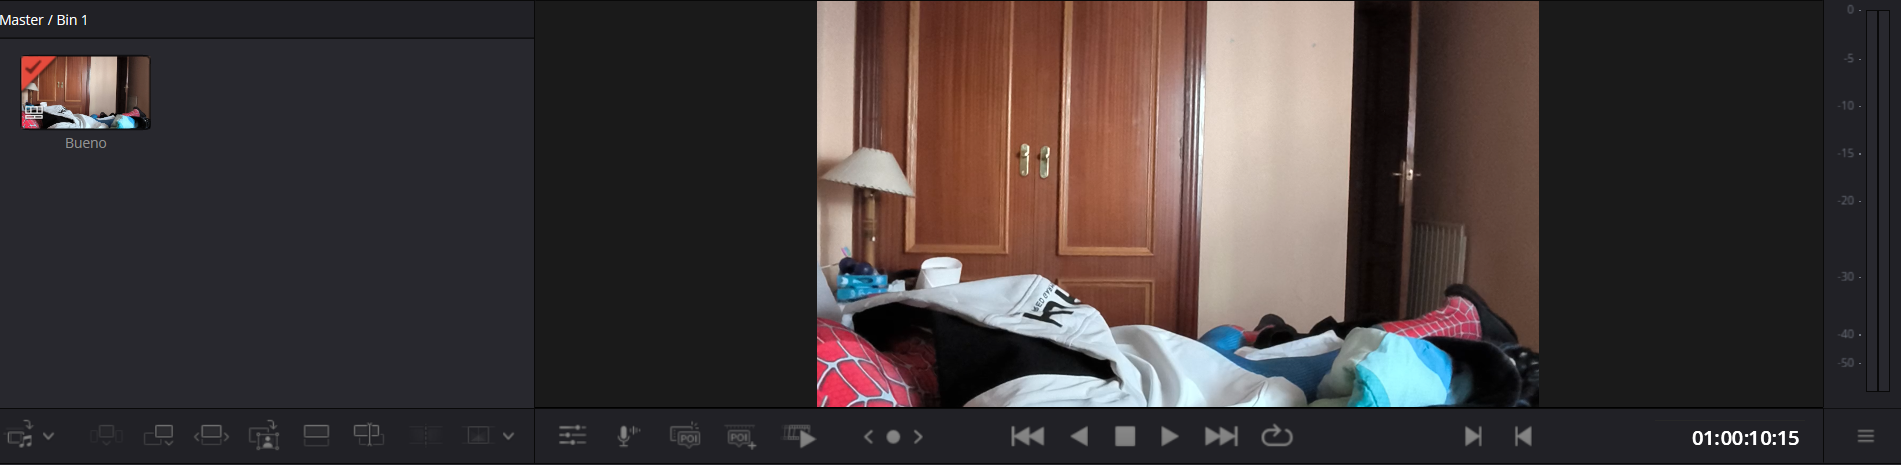
\includegraphics[width=1\textwidth]{assets/procesador_multimedia.png}
        \caption[Procesador Multimedia]{Procesador multimedia que dispone la interfaz\\ \footnotesize Fuente: Elaboración propia}
        \label{fig:procesador_multimedia}
    \end{figure}

    \item \textbf{Funcionalidades específicas}
    
    Esta sección, generalmente ubicada en paneles laterales o inferiores (véase Figura~\ref{fig:funcionalidad_especifica_1},
    ~\ref{fig:funcionalidad_especifica_2}), proporcionan acceso a herramientas especializadas que varían 
    en función del módulo activo. Incuye opciones para la edición de clips, ajustes de color, 
    incorporación de efectos, transiciones y manipulación del audio, entre otras.

    \begin{figure}[H]
        \centering
        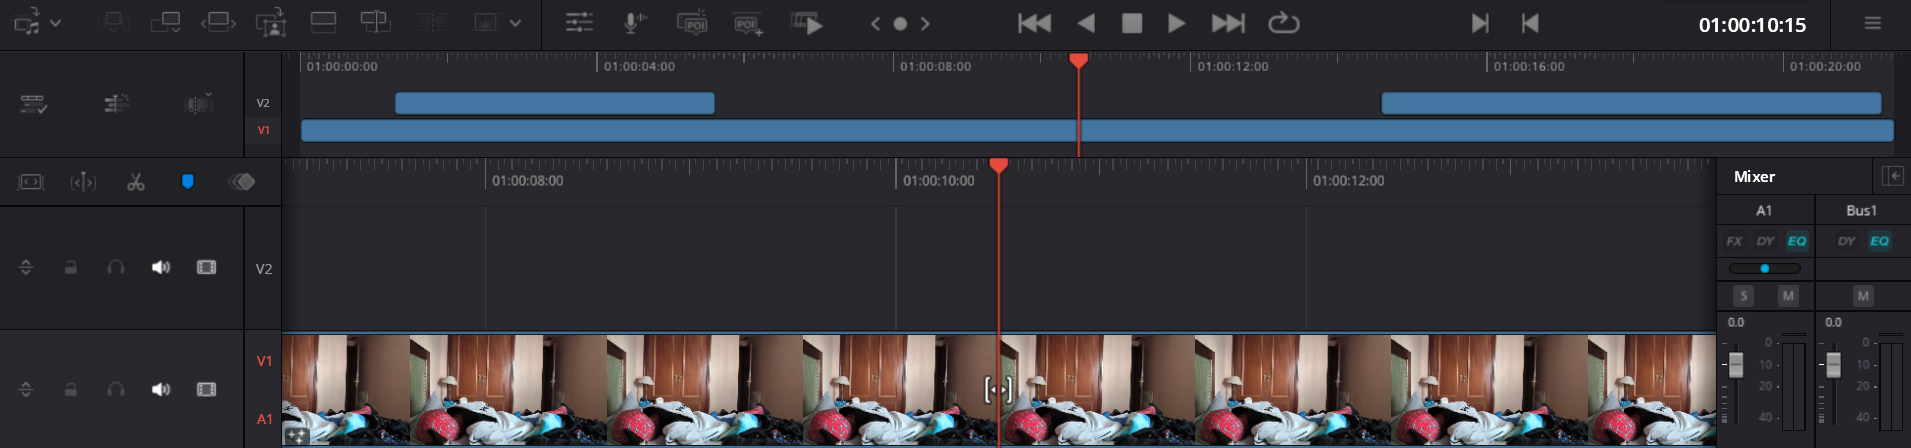
\includegraphics[width=1\textwidth]{assets/funcionalidad_especifica_1.png}
        \caption[Funcionalidades Especificas 1]{Funcionalidades especificas para las vistas de la interfaz\\ \footnotesize Fuente: Elaboración propia}
        \label{fig:funcionalidad_especifica_1}
    \end{figure}

    \begin{figure}[H]
        \centering
        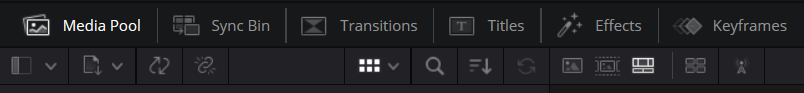
\includegraphics[width=1\textwidth]{assets/funcionalidad_especifica_2.png}
        \caption[Funcionalidades Especificas 2]{Funcionalidades especificas para las vistas de la interfaz\\ \footnotesize Fuente: Elaboración propia}
        \label{fig:funcionalidad_especifica_2}
    \end{figure}

\end{itemize}

\subsubsection{Módulos de trabajo}
\label{sec:modulos-trabajo}

Una de las características más relevantes de DaVinci Resolve es su organización en módulos o páginas 
de trabajo, cada una orientada a una fase concreta del proceso de edición:

\begin{itemize}
    \item \textbf{Media}: gestión e importación de archivos multimedia.
    \item \textbf{Cut}: edición rápida orientada a proyectos sencillos.
    \item \textbf{Edit}: edición con línea de tiempo avanzada.
    \item \textbf{Fusión}: creación de efectos visuales y composición.
    \item \textbf{Color}: correción y estalonaje de color profesional.
    \item \textbf{Fairlight}: edición y postproducción de audio.
    \item \textbf{Deliver}: exportación y renderización del proyecto final.
\end{itemize}

Esta estructura modular permite adaptar el flujo de trabajo a las necesidades específicas del proyecto, 
facilitando una organización clara y eficiente del proceso de edición (véase Figura~\ref{fig:modulos_trabajo}).

\begin{figure}[H]
    \centering
    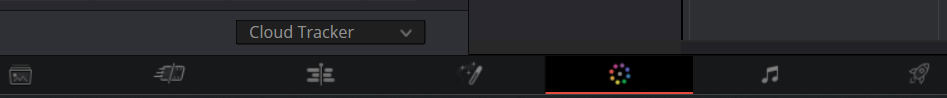
\includegraphics[width=1\textwidth]{assets/modulos_trabajo.png}
    \caption[Modulos trabajo]{Modulos de trabajo que ofrece DaVinci Resolve\\ \footnotesize Fuente: Elaboración propia}
    \label{fig:modulos_trabajo}
\end{figure}

\subsubsection{Importación y exportacion de contenido multimedia}
\label{sec:imp-exp}
Uno de los aspectos más importantes a tener en cuenta cuando se comienza a trabajar con la herramienta DaVinci 
es cómo podemos importar contenido multimedia para poder trabajar con él dentro de la herramienta y finalmente, 
cómo exportar el resultado creado.

Tras haber accedido a un proyecto creado en DaVinci, en la sección identificada anteriormente como 
\textbf{funcionalidades generales} se puede \textbf{importar} contenido multimedia a través de la opción 
\textbf{File -\textgreater Import -\textgreater Media} o mediante un atajo de teclados \textit{Ctrl + I}. Una vez importado el 
contenido, se puede trabajar con él tras incorporarlo a la línea temporal. El paso a seguir requiere seleccionar 
dicho contenido y 'arrastrarlo' a la línea temporal (véase Figura~\ref{fig:importar_contenido_linea}).

\begin{figure}[H]
    \centering
    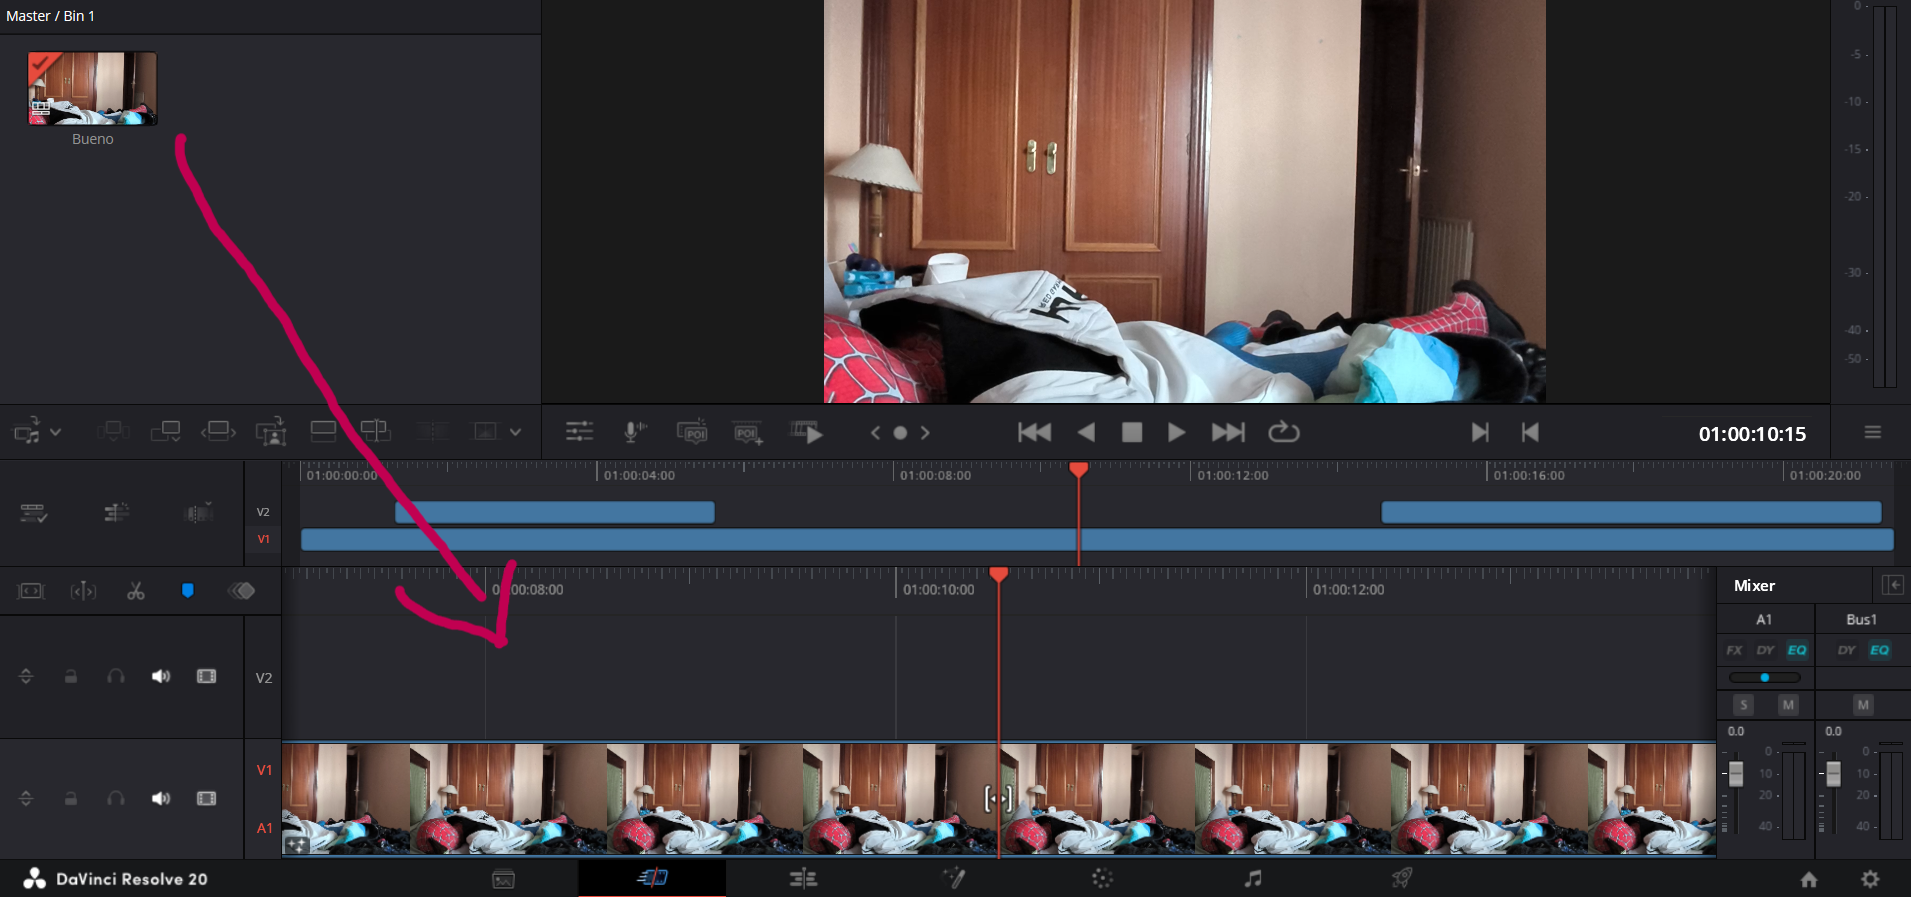
\includegraphics[width=1\textwidth]{assets/importar_multimedia.png}
    \caption[Importar Multimedia Linea Temporal]{Importar contenido multimedia a línea temporal\\ \footnotesize Fuente: Elaboración propia}
    \label{fig:importar_contenido_linea}
\end{figure}

La exportación de un vídeo editado se encuentra disponible gracias a la incorporación de un atajo visual en la interfaz de DaVinci. 
Se encuentra en la zona inferior de la interfaz, identificada con el símbolo de \textbf{cohete} en la Figura~\ref{fig:modulos_trabajo}.

Al acceder a ella, el programa presenta una interfaz de configuración(véase Figura~\ref{fig:exportacion_video}) sobre el formato de exportación 
que se aplicará al vídeo. Entre su configuración, se puede destacar la elección del tipo de \textit{códec}, resolución, 
calidad, entre otros. Una vez aplicada la configuración ideal a las características necesarias para el vídeo, 
se selecciona la opción \textbf{Add to Render Queue} y finalmente se selecciona la opción \textbf{Render All} (véase Figura~\ref{fig:exportacion_video}).

\begin{figure}[H]
    \centering
    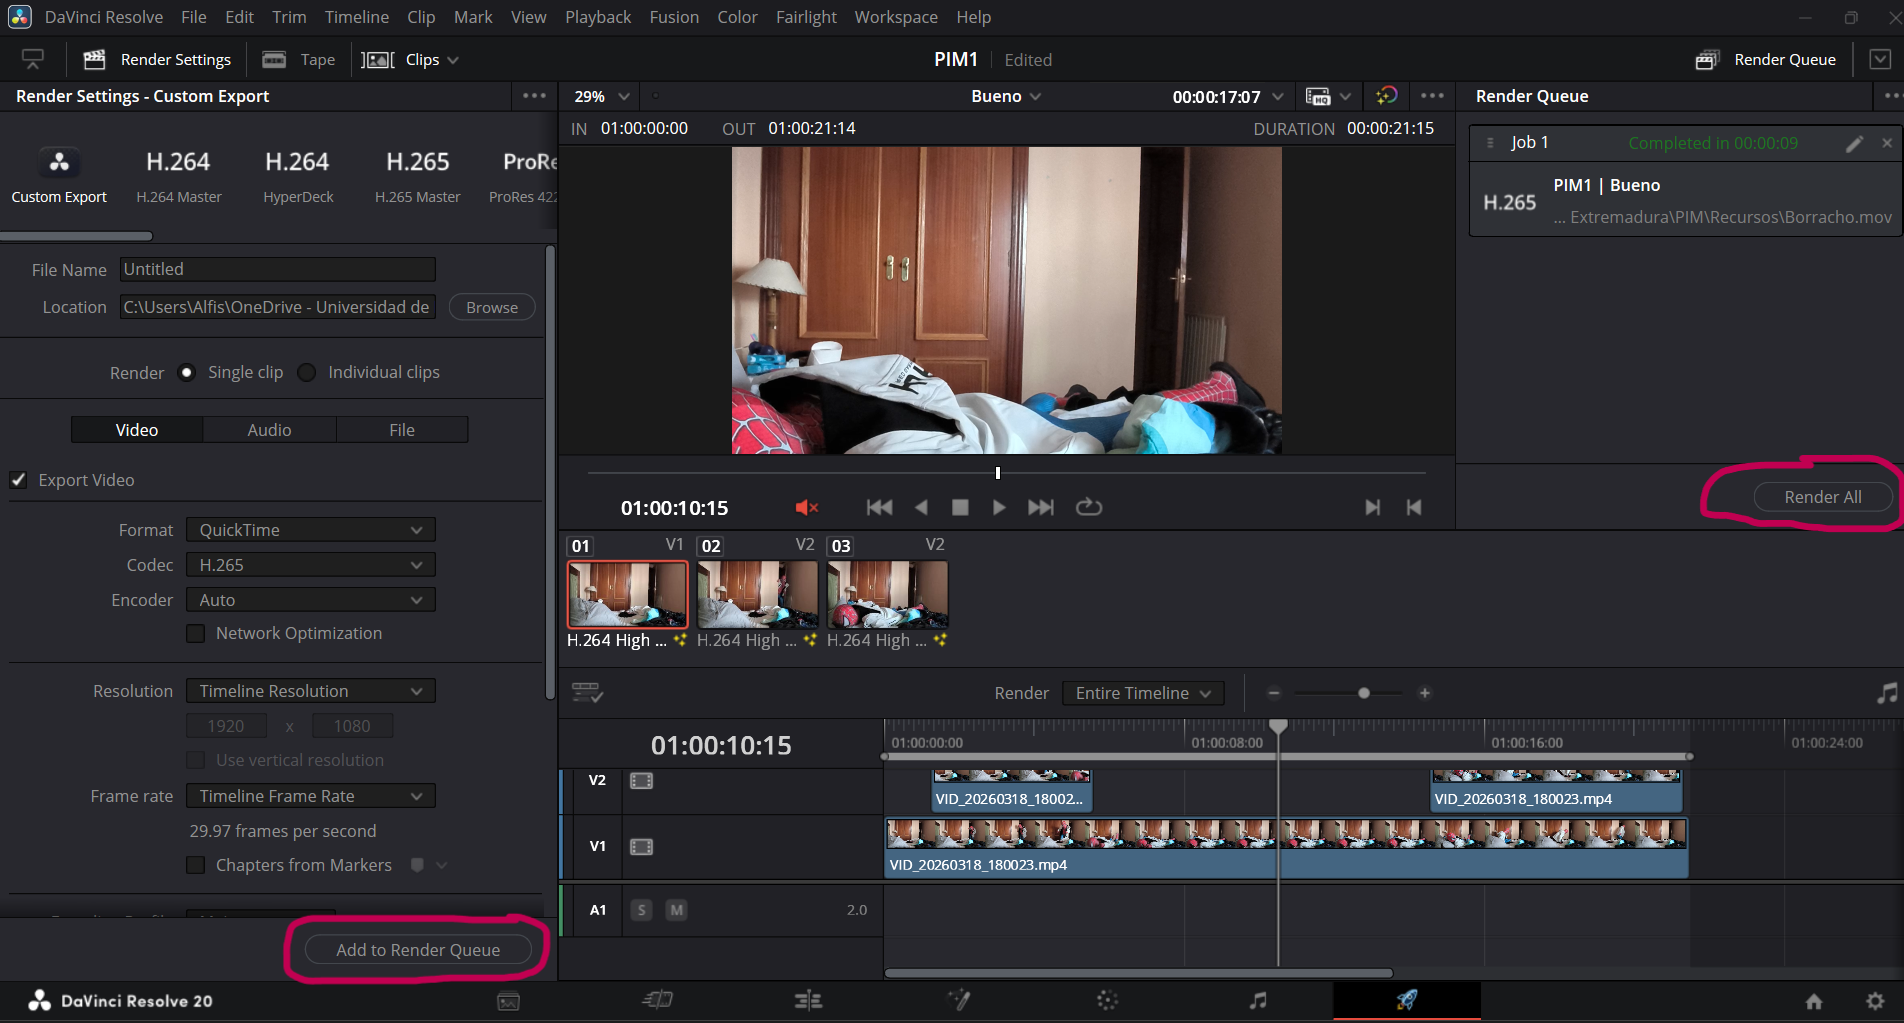
\includegraphics[width=1\textwidth]{assets/exportacion.png}
    \caption[Exportar video]{Ventana de exportación de vídeo\\ \footnotesize Fuente: Elaboración propia}
    \label{fig:exportacion_video}
\end{figure}

\subsection{Planificación de trabajo}
Antes de iniciar el desarrollo del proyecto, se dedicó una fase previa a la 
definición de la idea y del contexto, con el objetivo de establecer una base 
sólida sobre la que construir el resultado final. 

En esta subsección se describen, además, las distintas actividades llevadas 
a cabo durante cada una de las fases de grabación, permitiendo así comprender 
la organización y evolución del trabajo realizado.

\subsubsection{Ideas descartadas}
Antes de comenzar a grabar el vídeo, se generaron varias ideas sobre la temática del mismo, entre las cuales se descartaron aquellas que no se ajustaban 
a los objetivos del proyecto o que presentaban dificultades técnicas insuperables. Algunas de las ideas descartadas incluyen:

\begin{enumerate}
    \item \textbf{Escena de terror}
    
    Primeramennte se consideró la creación de una escena de terror utilizando efectos visuales y sonoros para generar una 
    atmósfera inquietante. Sin embargo, esta idea fue descartada rápidamente debido a que la correcta elaboración de la misma, dependía más
    de conocimientos propios sobre cine que de técnicas de edición de vídeo. Además, como desde el principio se quiso trabajar únicamente con
    vídeos grabados por los autores del proyecto, se consideró que esta idea no era viable debido a la falta de recursos y experiencia en la creación
    de este tipo de vídeos.

    La escena debería de tener también un sólido guión detrás, lo cual requeriría una planificación y esfuerzos adicionales que no se
    ajustaban al alcance del proyecto. Por estas razones, se decidió descartar esta idea y buscar otras opciones más adecuadas para el
    proyecto.

    \item \textbf{Trailer de superhéroes}
    
    Para no contar con el problema de tener que lidiar con la creación de un guión coherente que sustente la escena, se consideró la creación
    de un trailer de superhéroes. Utilizando como inspiración personajes populares de \textbf{Marvel} como \textit{Daredevil} o \textit{Punisher},
    los cuales no tienen grandes poderes díficiles de representar. Se pensó que una concatenación de escenas de acción, en el que se
    empleasen las técnicas de edición deseadas,sin necesidad de tener que manterner una coherencia narrativa.

    Se realizaron \textbf{esbozos} de un guión para el trailer. En la primera y única escena con diálogos del mismo, un héroe emergente, Din, iría
    en busca de un antiguo vigilante, Sam, altamente inspirado en \textit{Punisher}. Este último se encuentra retirado debido a que sus actividades
    heroicas le han llevado a perder a su familia a manos de un villano, \textbf{el Cuervo}. Din, trás descrubir el paradero del villano,
    pide ayuda a Sam para acabar con él. Trás esta breve introducción, se mostrarían una concatenación de escenas de acción en las que 
    se mostrarían las técnicas de edición deseadas. Muchas de estas ideas acabaron utilizandose en el proyecto final. Se propusieron
    varios nombres provisionales para esta idea (Véase Figura~\ref{fig:titulo-trailer}).

    \begin{figure}[H]
        \centering
        
\includegraphics[width=0.7\textwidth]{assets/titulo-trailer.png}
        \caption{Nombres para el trailer de superhéroes\\ \footnotesize Fuente: Elaboración propia con \textit{Nano Banana 2}}
        \label{fig:titulo-trailer}
    \end{figure}

    Sin embargo, esta idea también fue descartada debido a dificultades en las grabaciones. Aún optimizando al máximo los recursos disponibles,
    se requerían de varios días de grabación en el que ambos integrantes debían de quedar presencialmente con varios conjuntos de ropa diferentes,
    a cierta hora del día y con necesidad de recurrir a terceras personar para grabar escenas en las que apareciesen ambos integrantes. Dado
    que los horarios y disponibilidad de ambos integrantes no eran compatibles, se consideró que esta idea no era viable para el proyecto.



    \item \textbf{Tutorial de edición de vídeo}
Tras descartar varias ideas, se consideró que la opción más viable era la creación de un tutorial de edición de vídeo. Esta idea se basaba en la creación 
de un vídeo explicativo en el que se mostraran las técnicas de edición investigadas en el estado del arte. Las escenas a editar
serían rápidas de grabar, ya que se podrían grabar por separado y sin necesidad de recurrir a terceras personas. El vídeo 
incorporaría un \textbf{personaje animado} sencillamente en 2D que sería el encargado de explicar las técnicas de edición.
Aunque esta idea parecía asequible, se descartó debido a que se consideró que el resultado final no sería tan atractivo como otras
opciones. Se quiso optar por un proyecto más creativo y visualmente impactante.

\end{enumerate}

\subsubsection{Formalización de la idea}
Finalmente, debido a las limitaciones encontradas en las ideas anteriores, se decidió optar por un montaje con \textbf{tono humorístico}, inspirado en ciertos
vídeos encontrados en redes sociales. Donde un hombre, tras una ruptura amorosa, se da por vencido en la vida, cayendo en vicios
como el alcohol, las drogas o las apuestas. Se rescató un poco la idea del trailer de superhéroes, vistiendo al protagonista
del personaje \textbf{Spider-Man}, nunca dejando claro si es el propio héroe o alguien que se disfraza del mismo. Los efectos de vídeo
más psicódelicos se utilizaron para mostrar el estado mental del protagonista, mostrando su descenso a la locura.

El \textbf{ritmo} del vídeo consta claramente de dos partes diferenciadas. La primera, con un ritmo más pausado, en la que se muestra
la deprimente vida del protagonista acompañado de una música triste. La segunda parte, con un ritmo mucho más frenético, 
en la que tras consumir ciertas drogas, se concatenan un gran despliegue de efectos y técnicas visuales,
acompañado de una música más agresiva. En referencia a las últimas películas del personaje como \textit{Homecoming}, \textit{Far From Home} o
\textit{No Way Home}, se optó por el título \textbf{Spider-Man: Home-less}.(Véase Figura~\ref{fig:Spiderman-homeless}).

\begin{figure}[H]
    \centering
    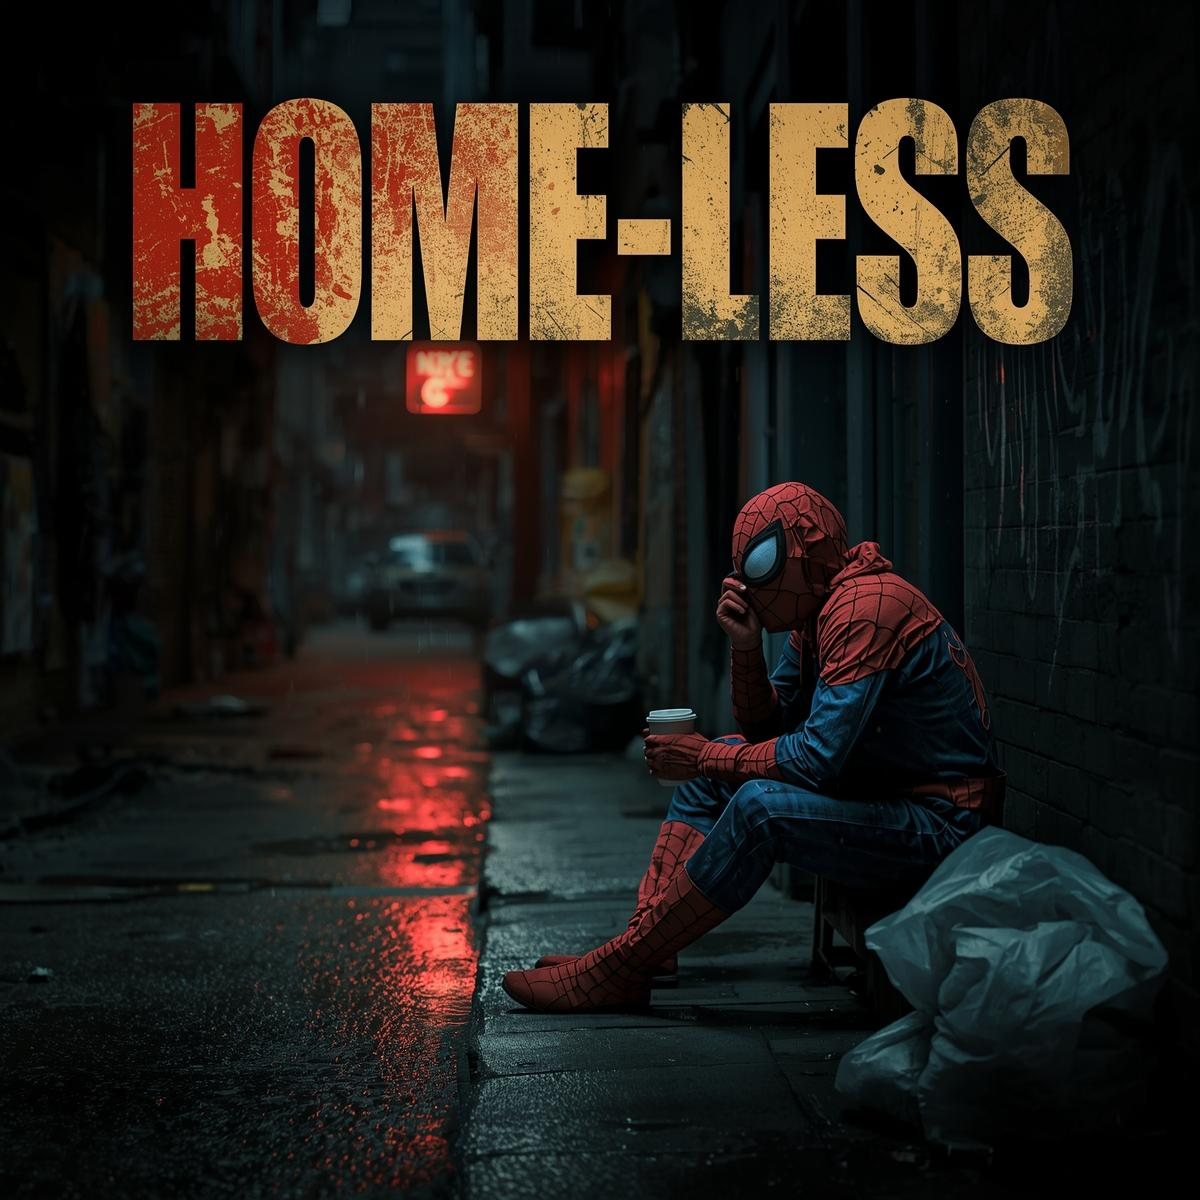
\includegraphics[width=0.5\textwidth]{assets/Spider-man-Home-less.jpg}
    \caption{Concept art generado con IA\\ \footnotesize Fuente: Elaboración propia con \textit{Nano Banana 2}}
    \label{fig:Spiderman-homeless}
\end{figure}

Se optó por esta idea ya que la mayoría de escenas podían ser grabadas en solitario desde casa, donde ya se disponía
de la mayor parte de los recursos necesarios.


\subsubsection{Grabación}
Una de las partes más satisfactorias del proyecto fue la grabación de las escenas. Se utilizó la cámara del móvil de uno de los
integrantes, la cámara de un \textit{POCO X7 pro}, sin ser el fuerte del teléfono, captura vídeos con su cámara interna a 1080p y 30fps,
la calidad originalmente planificada para el vídeo. Tambien se tomaron fotografías para capturar el proceso de creación del vídeo.
Asimismo, se planteó la inclusión de las fotografías en el vídeo, pero se descartó por la falta de ritmo.
 Se planificaron originalmente \textbf{dos días de grabación},uno para cada parte del vídeo. Las primera parte, más pausada, se grabó en interiores, en el piso de uno de los integrantes.
La mayoría de los planos en esta parte son \textbf{estáticos}, con el protagonista sentado o tumbado en el sofá, 
mostrando su estado de ánimo deprimente. Siempre hay algún objeto dañino para la salud en pantallas, como botellas de alcohol 
o cigarrillos (Véase Figura~\ref{fig:Grabacion-parte1}). 

\begin{figure}[H]
    \centering
    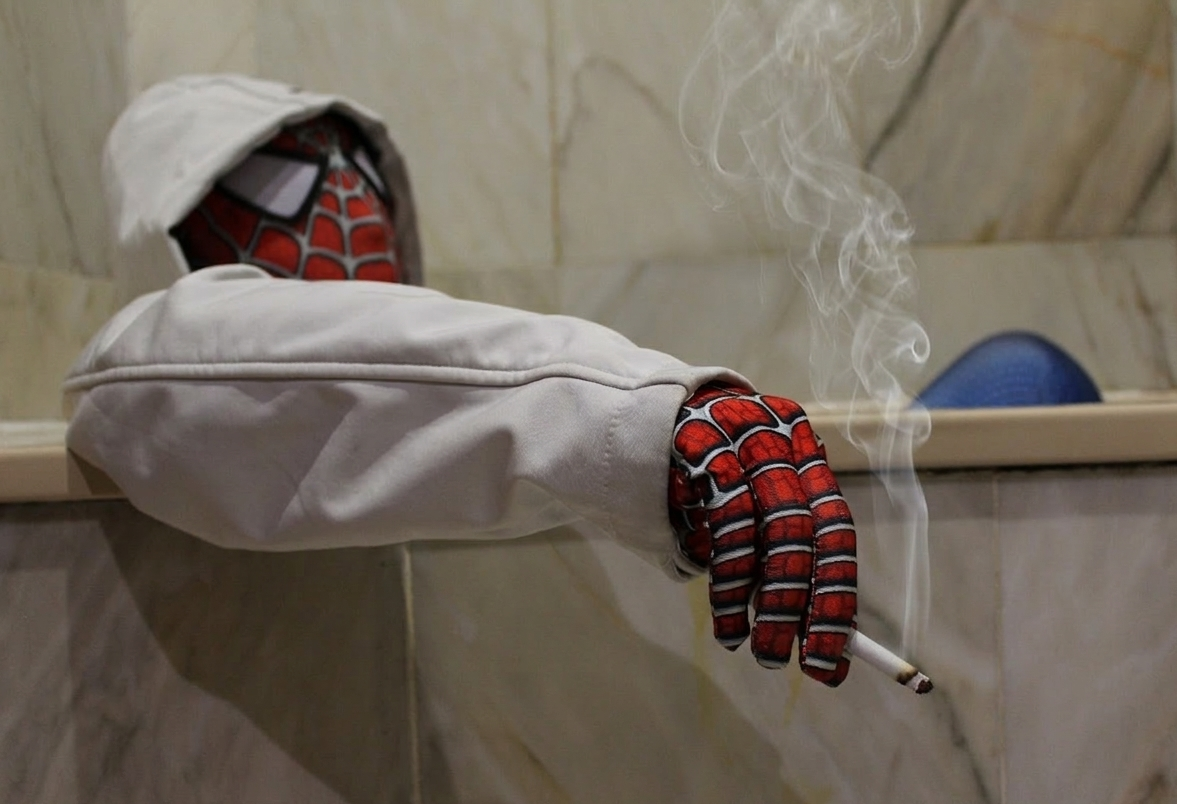
\includegraphics[width=0.7\textwidth]{assets/Grabacion-parte1.png}
    \caption{Primer día de grabación\\ \footnotesize Fuente: Elaboración propia}
    \label{fig:Grabacion-parte1}
\end{figure}

Mientras que la segunda parte, más \textbf{frenética}, se grabó en exteriores. Permitiendo así una mayor movilidad y posibilidades
para la inclusión de los efectos visuales, más presentes en esta parte. Finalmente se necesitaron de dos días para
completar las tomas deseadas, pues el tiempo de metraje grabado era inferior al esperado. Tampoco se tuvo en cuenta el tiempo necesario
para trasladarse entre las distintas localizaciones, las cuales estaban bastante dispersas entre ellas.
El segundo día de grabación se realizaron las escenas transición entre la primera y segunda parte, la mayoría en entornos urbanos. (véase Figura~\ref{fig:Grabacion-parte2}). 
Se aprovechó de la luz natural para tener una mejor iluminación, un tema que había dado problemas hasta ese momento. Se descartaron
algunas ideas iniciales como un atraco u otras referencias a las películas originales del personaje, debido a la necesidad de contar
con bastantes personas para poder realizarse correctamente.

\begin{figure}[H]
    \centering
    \includegraphics[width=0.5\textwidth]{assets/Grabacion-parte2.jpg}
    \caption{Segundo día de grabación\\ \footnotesize Fuente: Elaboración propia}
    \label{fig:Grabacion-parte2}
\end{figure}

El tercer día, no planificado inicialmente, se utilizó para grabar las escenas finales del vídeo. Se pensó en localizaciones más en contacto
con la naturaleza para darle un toque más espiritual, como si el camino del personaje hubiera sido una peregrinación.
 La mayoría de ellas se grabaron a las afueras de la ciudad. Se utilizó otra vestimenta con respecto a las anteriormente grabadas. 
 El protagonista en este punto no distingue la realidad de la ficción, inspirado por 
otros personajes de comics dementes como Joker o Deadpool (Véase Figura~\ref{fig:Grabacion-parte3}). Tambien se aprovechó
para grabar algunos recursos como saltos o caídas, necesarios para hacer algunos de los efectos visuales.

\begin{figure}[H]
    \centering
    \includegraphics[width=0.6\textwidth, angle=-90]{assets/Grabacion-parte3.JPG}
    \caption{Tercer día de grabación\\ \footnotesize Fuente: Elaboración propia}
    \label{fig:Grabacion-parte3}
\end{figure}


\subsubsection{Desarrollo}
El desarrollo del proyecto se estructura en dos bloques principales, cada uno enfocado a una parte 
clave del proceso de edición audiovisual.

Por un lado, se aborda el montaje del vídeo, centrado en la organización y sincronización de los distintos 
clips grabados para conformar una secuencia continua coherente, ajustada al ritmo y compás de la música 
seleccionada. Esta fase incluye la selección de tomas, su ordenación y la definición del tempo narrativo del 
vídeo.

Por otro lado, se desarrollan los efectos visuales aplicados a cada clip, con el objetivo de enriquecer 
la narrativa visual y, en determinados casos, incorporar elementos que 
no pueden ser capturados directamente durante la grabación. Esta fase implica el uso de técnicas de 
postproducción para transformar y mejorar el material original.
\subsection{Montaje}
El montaje del vídeo fue el proceso inicial de edición, en el que se organizaron los clips grabados para conformar una secuencia coherente.
Proceso muy importante, ya que sentó las bases para el desarrollo de los efectos visuales posteriores. 

Inicialmente, se grabaron las escenas sin tener claro la música que las acompañaría despues, por lo que el primer trabajo fue seleccionar
la banda sonora que mejor se ajustara a la narrativa visual que se quería contar. Eran necesarios dos temas musicales con tonos distintos,
uno para cada parte del video. Se estimaron unos 6-7 minutos de metraje útil para utilizar. Para la primera se eligió In the pool, procedente
de la banda sonora de la película Chainsaw Man – The Movie: Reze Arc (véase Figura~\ref{fig:musica1}), que encajaba perfectamente con el tono
y duración deseados.

\begin{figure}[H]
    \centering
    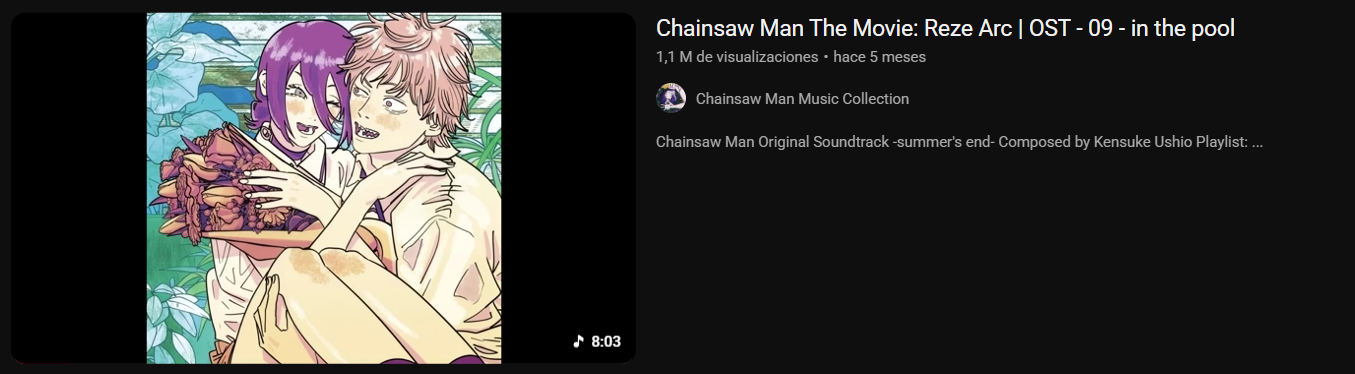
\includegraphics[width=1\textwidth]{assets/musica1.png}
    \caption{Selección de la música para la primera parte del vídeo\\ \footnotesize Fuente: Elaboración propia}
    \label{fig:musica1}
\end{figure}

La música es posiblemente el elemento más importante a la hora de marcar el ritmo del vídeo, la mayoría de los cortes
realizados se hicieron siguiendo el compás de la música. Es un proceso técnicamente sencillo, (véase Figura~\ref{fig:montaje1}),
pero que requiere de una gran atención y paciencia para conseguir un resultado satisfactorio. 


Para la segunda parte del vídeo, más animada, se eligió un frafmento del tema Epilogue, procedente de la bandara sonora de la película
La La Land (véase Figura~\ref{fig:musica2}). Esta elección fue más complicada, ya que se contemplaban múltiples
opciones, la mayoría más frenéticas que esta. Pero para este punto ya había una mejor idea del resultado final del vídeo y
esta música era la que mejor encajaba con algunos de los efectos que se querían aplicar, y de los que se hablarán a continuación.
La idea del montaje era completar la columna vertebral del vídeo, una versión 0 sobre la que ir trabajando e iterando con los 
efectos visuales y pequeños retoques, pero con la certeza de que el resultado final no se distanciaría demasiado del concepto 
original.

\begin{figure}[H]
    \centering
    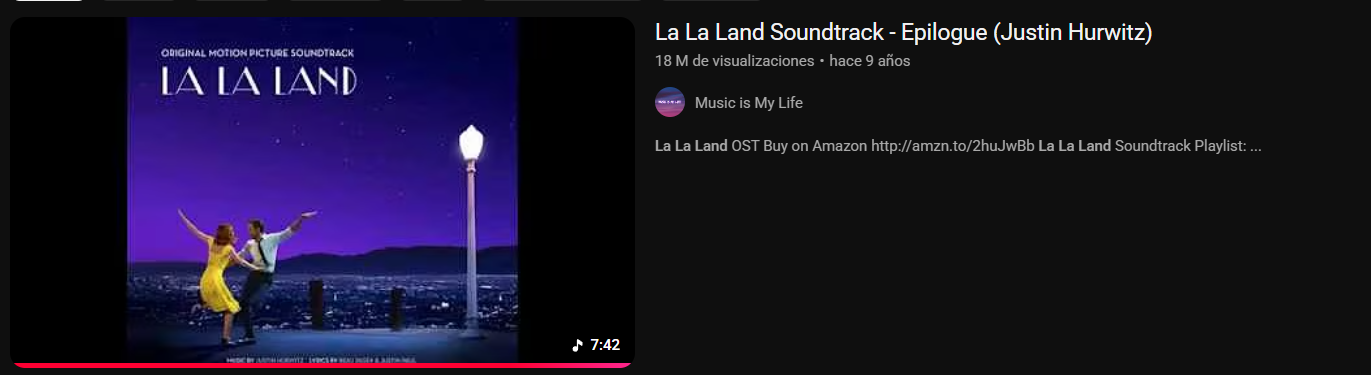
\includegraphics[width=1\textwidth]{assets/musica2.png}
    \caption{Selección de la música para la segunda parte del vídeo\\ \footnotesize Fuente: Elaboración propia}
    \label{fig:musica2}
\end{figure}

Para realizar el montaje de un vídeo, se debe de arrastrar los clips de los que 
se quiere disponer a la línea temporal. Despues, se procederá a cortar las partes
no necesarias de cada clip. En Davinci Resolve, al presionar la tecla \textit{B}, 
se activa la herramienta de corte, que permite dividir donde se pinche con el ratón. Después
hay que pulsar la tecla \textit{A} para volver a la herramienta de selección, 
con la que se seleccionan los fragmentos a eliminar con la tecla \textit{Retroceso}. Esta es
una manera válida, pero es más rápido utilizar el atajo de teclado \textit{Ctrl + B} para 
cortar el clip directamente sin necesidad de cambiar de herramienta.

En nuestro vídeo no se quiere que haya audio procedente de los clips, esto se conseigue haciendo
click derecho sobre el clip, seleccionando la opción \textbf{Link Clips} para desvincular el audio
del vídeo, y posteriormente eliminando el audio con la tecla \textit{Retroceso}. También se puede 
hacer directamente con el atajo de teclado \textit{Ctrol + Alt + L}. Simplemente aplicando estos
dos conceptos y añadiendo la música de fondo, ya se puede conseguir el montaje básico, necesario
para conseguir esa versión 0 de la que hablábamos.

\begin{figure}[H]
    \centering
    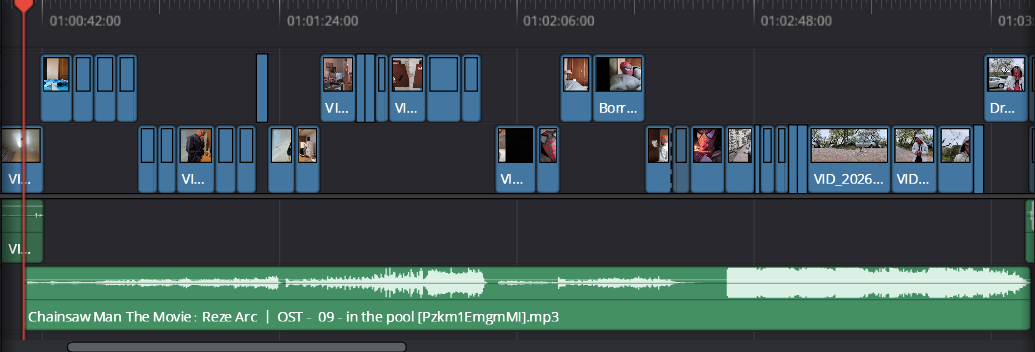
\includegraphics[width=1\textwidth]{assets/montaje1.png}
    \caption{Montaje de la primera parte del vídeo\\ \footnotesize Fuente: Elaboración propia}
    \label{fig:montaje1}
\end{figure}


\subsection{Efectos especiales}

Todos los efectos detallados a continuación comparten la funcionalidad de selección e importación de un clip de vídeo a editar en la 
línea de tiempo (véase Sección~\ref{sec:imp-exp}) \textcolor{importante}{IMPORTANTE}.

\subsubsection{Brillo y rayos de luz}

Este efecto se caracteriza por la intensificación de la iluminación presente en el clip, 
generando una sensación de deslumbramiento a partir de una fuente de luz artificial. 
En el caso aplicado, se parte de la luz natural emitida por una lámpara de dormitorio, 
la cual se transforma en una ráfaga de luz más intensa.

\textbf{Pasos seguidos para la aplicación del efecto:}
\begin{enumerate}[label=\arabic*.]

    \item \textbf{Importación del efecto al clip}: Para aplicar el efecto que permite alcanzar el objetivo propuesto, es necesario 
    acceder al apartado \textbf{Color} (véase Sección~\ref{sec:modulos-trabajo}, Figura~\ref{fig:modulos_trabajo}). Una vez dentro, 
    se selecciona el nodo asociado al vídeo (véase Figura~\ref{fig:light-effect}, Opción 1) y, a continuación, el apartado \textbf{Effects} 
    situado en la parte superior derecha de la interfaz. Posteriormente, se busca mediante la \textbf{lupa} el 
    efecto \textit{Light Rays} (véase Figura~\ref{fig:light-effect}, Opción 2)y, una vez localizado, se arrastra 
    sobre el nodo previamente seleccionado.

    \item \textbf{Viveza progresiva}: Tras aplicar el efecto, su configuración interna aparece automáticamente en el mismo apartado 
    de la interfaz donde fue seleccionado. En esta fase, se establecen valores específicos en determinados instantes del clip con el 
    objetivo de obtener un resultado natural.

    Un aspecto \textcolor{importante}{importante} es el uso de \textit{KeyFrames}, definidos como puntos clave en la línea de 
    tiempo que marcan el inicio y el fin de una variación en los parámetros del efecto. Sin su utilización, el efecto permanecería 
    activo de forma constante durante todo el clip, lo cual no se ajusta al objetivo buscado.

    Para ello, en la misma sección de la interfaz, se dispone de una línea temporal en la parte inferior derecha denominada 
    \textbf{KeyFrames} (véase Figura~\ref{fig:light-effect}, Opción 3). En ella, se posiciona la \textbf{barra roja} en el instante en el que se desea iniciar el efecto, se hace 
    clic derecho y se selecciona la opción \textit{Add Dynamic KeyFrame}. Este mismo proceso se repite para el instante en el que se 
    desea finalizar el efecto.

    \item \textbf{Reajuste de valores}:
    Una vez definidos estos dos puntos temporales, se ajustan los valores del efecto en cada uno de ellos. En este caso, se 
    establecen valores mínimos en el instante inicial y valores más elevados en el instante final, generando una transición 
    progresiva del brillo que produce un resultado más natural y visualmente atractivo.

    \item \textbf{Recomendaciones}:
    ¿Por qué se utiliza un \textit{KeyFrame} \textbf{dinámico} en lugar de uno \textbf{estático}? Como se ha descrito, el uso de valores diferentes 
    en los instantes inicial y final permite que, a medida que transcurre el tiempo entre ambos, los parámetros evolucionen de forma 
    progresiva. Esto aporta mayor fluidez y calidad visual al clip. Por el contrario, el uso de \textit{KeyFrames} estáticos provoca 
    cambios bruscos en los valores, generando transiciones poco naturales que pueden resultar desagradables para el espectador.

    \begin{figure}[H]
        \centering
        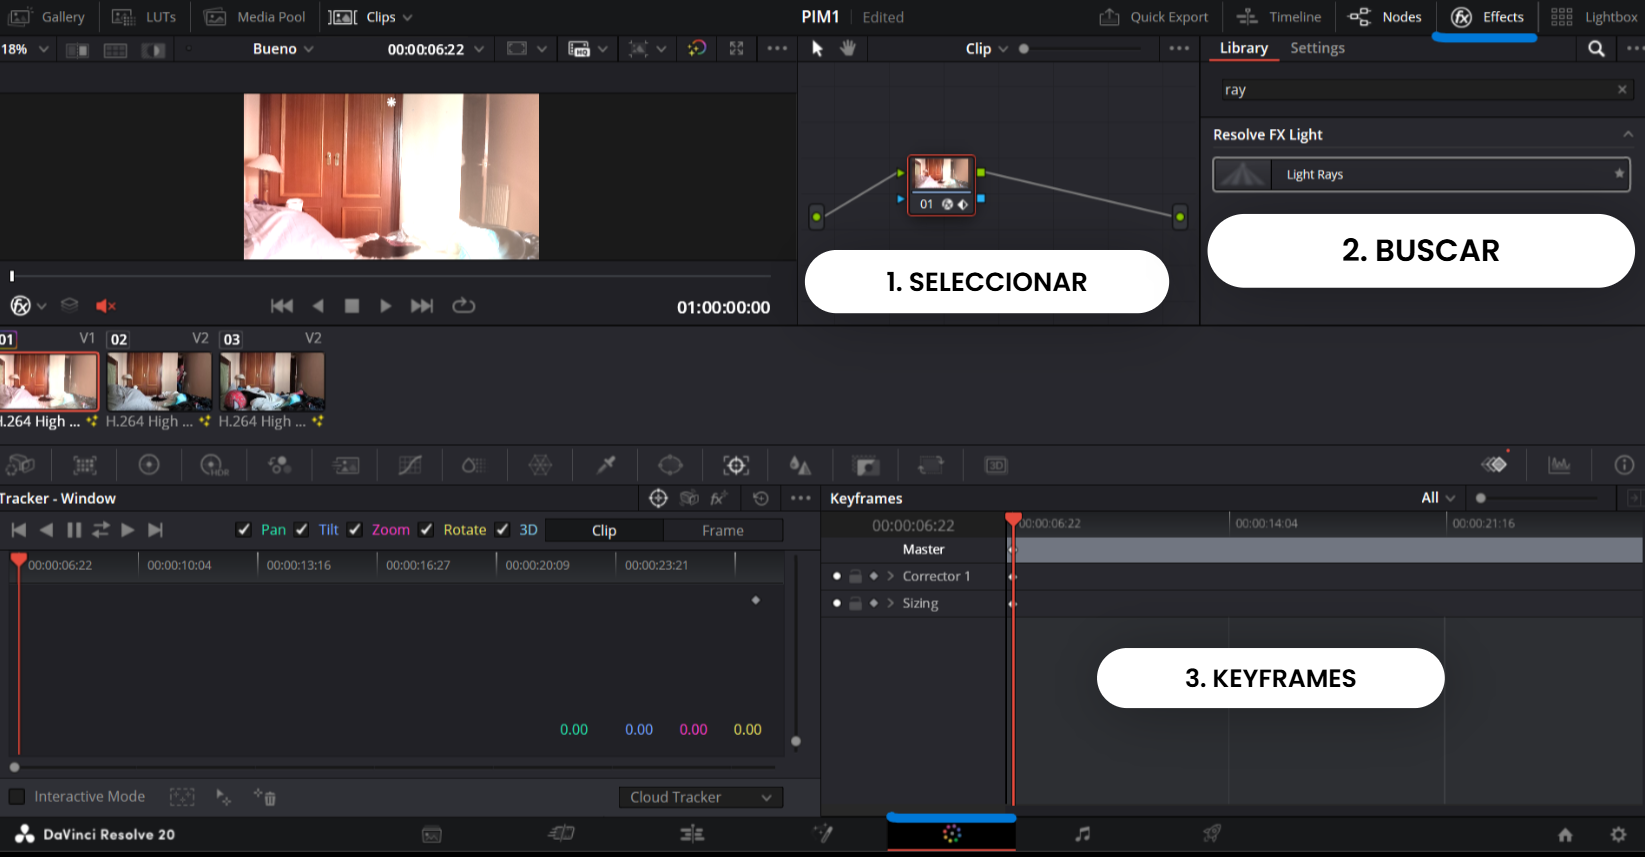
\includegraphics[width=1\textwidth]{assets/light-effect.png}
        \caption[Primer efecto]{Creación de Light-Effect\\ \footnotesize Fuente: Elaboración propia}
        \label{fig:light-effect}
    \end{figure}
\end{enumerate}

\subsubsection{Detector de cabeza y \textit{drunk} effects}

Este efecto se caracteriza por la incorporación de un detector de cabezas junto con una visión doble aplicada sobre 
un elemento del vídeo, en este caso, una persona. En el escenario planteado, se parte de un clip estático en el que una persona 
realiza diversos movimientos, generando como resultado una sensación de movimiento dinámico de cámara, similar a un efecto de mareo.

\textbf{Pasos seguidos para la aplicación del efecto:}
\begin{enumerate}[label=\arabic*.]

    \item \textbf{Importación del efecto al clip}: Para aplicar el efecto deseado, es necesario acceder al apartado \textbf{Fusion}
        (véase Sección~\ref{sec:modulos-trabajo}, Figura~\ref{fig:modulos_trabajo}). Una vez dentro, se debe ubicar la pestaña inferior 
        izquierda denominada \textbf{Nodes}, donde se representan los nodos encargados de gestionar el flujo de entrada y salida.

    Por defecto, aparecen dos nodos inicializados: \textit{MediaIn1} (contenido de entrada) y \textit{MediaOut1} (resultado final), 
    los cuales se encuentran conectados entre sí. Esta estructura permite la incorporación de nodos intermedios que actúan como 
    \textbf{efectos o filtros}.

    La simulación del movimiento dinámico sobre un vídeo estático se consigue mediante el seguimiento en tiempo de ejecución 
    de la cabeza de la persona. Para ello, se emplea el nodo \textbf{PlanarTracker}. Su incorporación se realiza seleccionando el 
    nodo \textit{MediaIn1} y utilizando el atajo \textit{Shift + Espacio}, que abre el buscador de efectos. A continuación, se 
    busca \textbf{Planar Tracker}, se selecciona y se añade mediante la opción \textbf{Add}.

    El nuevo nodo debe aparecer en la vista \textit{Nodes}, correctamente enlazado entre \textit{MediaIn1} y \textit{MediaOut1}.

    \item \textbf{Configuración de Planar Tracker}: Una vez añadido el nodo, es necesario configurarlo definiendo una región de 
    interés (ROI) sobre la cabeza de la persona. Para ello, se selecciona el nodo \textit{PlanarTracker1} en la vista \textit{Nodes}. 
    En el panel derecho de la interfaz se muestran sus opciones de configuración, donde se pueden ajustar parámetros como el tipo de 
    detección (\textit{Tracking}) y el tipo de movimiento (\textit{Motion Type}).

    En este caso, se selecciona el tipo de detección por puntos (\textit{Points}) y el tipo de movimiento \textit{Translation}, lo que 
    permite al sistema aprender los desplazamientos mediante traslaciones (véase Figura~\ref{fig:config_planar}).

    \begin{figure}[H]
        \centering
        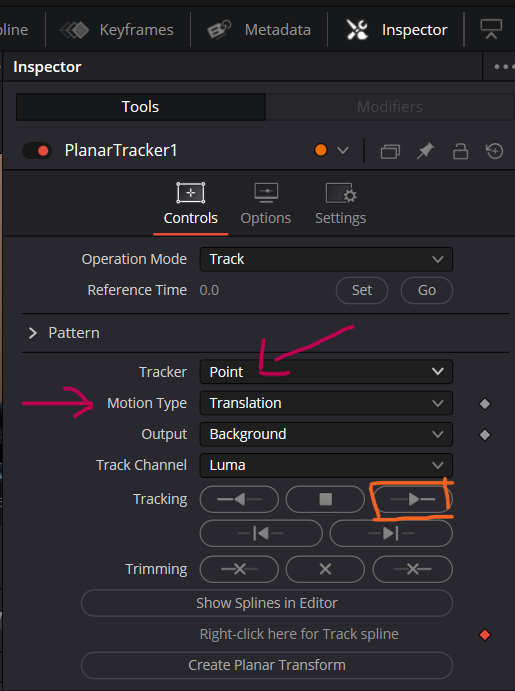
\includegraphics[width=0.4\textwidth]{assets/config_planar.png}
        \caption[Planar Tracker]{Configuración Base de Planar Tracker\\ \footnotesize Fuente: Elaboración propia}
        \label{fig:config_planar}
    \end{figure}

    Posteriormente, en la vista del vídeo, se debe definir un \textbf{polígono} mediante clics izquierdos que delimite la cabeza de 
    la persona (véase Figura~\ref{fig:poligono_tracker}). Es \textcolor{importante}{importante} realizar este proceso en el instante \textbf{0.0} del vídeo. En caso de que la 
    cabeza no sea visible en ese instante, se puede definir el polígono en una posición aproximada, ya que el sistema se encargará de 
    ajustarlo automáticamente durante el seguimiento.

    \begin{figure}[H]
        \centering
        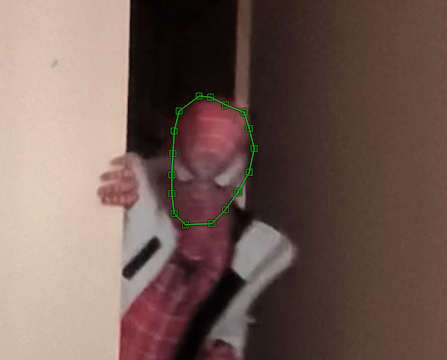
\includegraphics[width=0.6\textwidth]{assets/poligono_tracker.png}
        \caption[Crear ROI]{Creación de la ROI para la detección de movimiento\\ \footnotesize Fuente: Elaboración propia}
        \label{fig:poligono_tracker}
    \end{figure}

    \item \textbf{Ejecución del reconocimiento}: Una vez definido el polígono de detección, se procede a ejecutar el seguimiento del 
    movimiento a lo largo de todo el clip. Para ello, se utiliza la opción \textbf{-\textgreater-} dentro de la sección \textit{Tracking}. 
    Esta acción reproduce automáticamente el vídeo, permitiendo al sistema analizar frame a frame la posición de la cabeza.

    Al finalizar el proceso, es posible reproducir el resultado desde otros apartados como \textbf{Cut} 
    (véase Sección~\ref{sec:modulos-trabajo}, Figura~\ref{fig:modulos_trabajo}) para comprobar el comportamiento del efecto aplicado.


    \item \textbf{Efecto \textit{drunk}}: Sobre el mismo clip, se continúa trabajando desde el apartado \textbf{Edit} 
    (véase Sección~\ref{sec:modulos-trabajo}, Figura~\ref{fig:modulos_trabajo}). Una vez dentro, se realiza una duplicación del 
    clip presente en la línea de tiempo mediante \textbf{Copia - Pega} (\textit{Ctrl+C - Ctrl+V}).

    Posteriormente, el clip duplicado se arrastra sobre el clip original, situándolo en una pista superior. 
    A continuación, se selecciona el clip duplicado y, desde el panel de propiedades (ubicado en la parte superior derecha), 
    se accede a la sección \textbf{Composite}, donde se ajusta la subpropiedad \textit{Opacity} al valor 50.0.

    Finalmente, se modifica la propiedad \textbf{Speed Change}, ajustando la subpropiedad \textit{Change Speed} a 95.0. 
    Esta combinación de superposición, transparencia y ligera variación en la velocidad genera el efecto visual de visión doble y 
    distorsión característico del efecto \textit{drunk} (véase Figura~\ref{fig:drunk}).

    \begin{figure}[H]
        \centering
        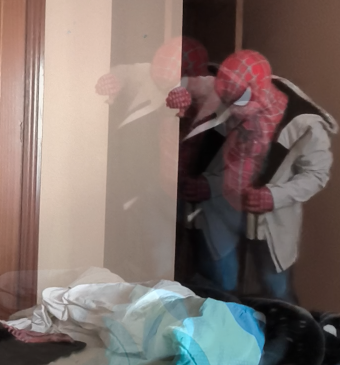
\includegraphics[width=0.4\textwidth]{assets/drunk.png}
        \caption[Efecto drunk]{Efecto \textit{drunk}\\ \footnotesize Fuente: Elaboración propia}
        \label{fig:drunk}
    \end{figure}
\end{enumerate}

\subsubsection{Efecto door loop}
    
El objetivo de este efecto es sorprender al espectador mediante la superposición de múltiples puertas dentro de un mismo vídeo. 
Estas puertas son abiertas por una misma persona y se sitúan próximas entre sí, pero con diferentes ángulos, generando la sensación 
de que el actor se observa a sí mismo en un mismo espacio vacío en varias posiciones simultáneamente. Este planteamiento produce un 
efecto visual similar a un espejismo.

\textbf{Pasos seguidos para la aplicación de este efecto:}
\begin{enumerate}[label=\arabic*.]
    \item \textbf{Ajuste inicial sobre el vídeo multimedia}
    
    Tras importar e incorporar el archivo multimedia a la línea temporal, resulta conveniente recortarlo seleccionando como instante 
    inicial el momento aproximado en el que el actor comienza a abrir la puerta, y como instante final aquel en el que la cierra, 
    desde el apartado \textbf{Cut} (véase Sección~\ref{sec:modulos-trabajo}, Figura~\ref{fig:modulos_trabajo}).

    Una vez obtenido el clip resultante, es posible que las acciones de apertura y cierre resulten algo bruscas o poco naturales, 
    por lo que se recomienda suavizarlas.

    Para ello, se emplean técnicas de \textbf{fundido de entrada y salida} (\textit{fade in} y \textit{fade out}). Se selecciona el 
    clip recortado y, a continuación, se ajustan las marcas visuales situadas en las esquinas superiores del clip (véase Figura~\ref{fig:fade_in_out}), 
    desplazándolas ligeramente hacia el interior mediante clic y arrastre con el ratón.

    Tras aplicar estos ajustes, se consigue que las acciones de apertura y cierre comiencen desde un negro absoluto y evolucionen de 
    forma progresiva, logrando una transición más suave y natural en el desarrollo del clip.

    Seguidamente, es necesario crear un clip de fusión (clic derecho en el clip -\textgreater \textit{New Fusion Clip}) 
    que contendrá este ajuste aplicado y permitirá trabajará con él como una entidad única para conseguir el efecto esperado.

    \begin{figure}[H]
        \centering
        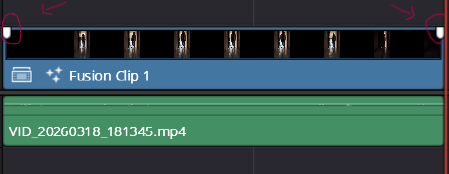
\includegraphics[width=1.0\textwidth]{assets/fade_in_out.png}
        \caption[Fadein-out]{\textit{Fade in} y \textit{Fade out} sobre el clip de vídeo\\ \footnotesize Fuente: Elaboración propia}
        \label{fig:fade_in_out}
    \end{figure}

    \item \textbf{Configuración del entorno de trabajo}
    
    Al crear el clip de fusión, se procede a configurar su disposición en el lienzo de trabajo. Para ello, es necesario acceder al apartado 
    \textbf{Fusion} (véase Sección~\ref{sec:modulos-trabajo}, Figura~\ref{fig:modulos_trabajo}). En él, observamos la vista de la interfaz 
    dedicada a los nodos situada en la parte inferior de la misma. Se selecciona el nodo \textit{MediaIn1} y en la barra de herramientas 
    que se puede aplicar a los nodos, ubicada justo encima de la vista de nodos, se selecciona la opción \textit{Rectangle}, conectándola 
    con el \textit{MediaIn1}.

    A continuación viene un proceso tedioso. Se debe ajustar el rectángulo en la vista del editor de vídeo ubicada en la parte central de la 
    interfaz, siendo sus límites delimitados por el marco de la puerta. Si no se obtiene una buena referencia para ajustar el clip sobre estas 
    consideraciones indicadas, es recomedable adelantar el clip hasta un instante de tiempo que permita obtener correctamente las referencias 
    (véase Figura~\ref{fig:rectangle_puertas}).
    
    \begin{figure}[H]
        \centering
        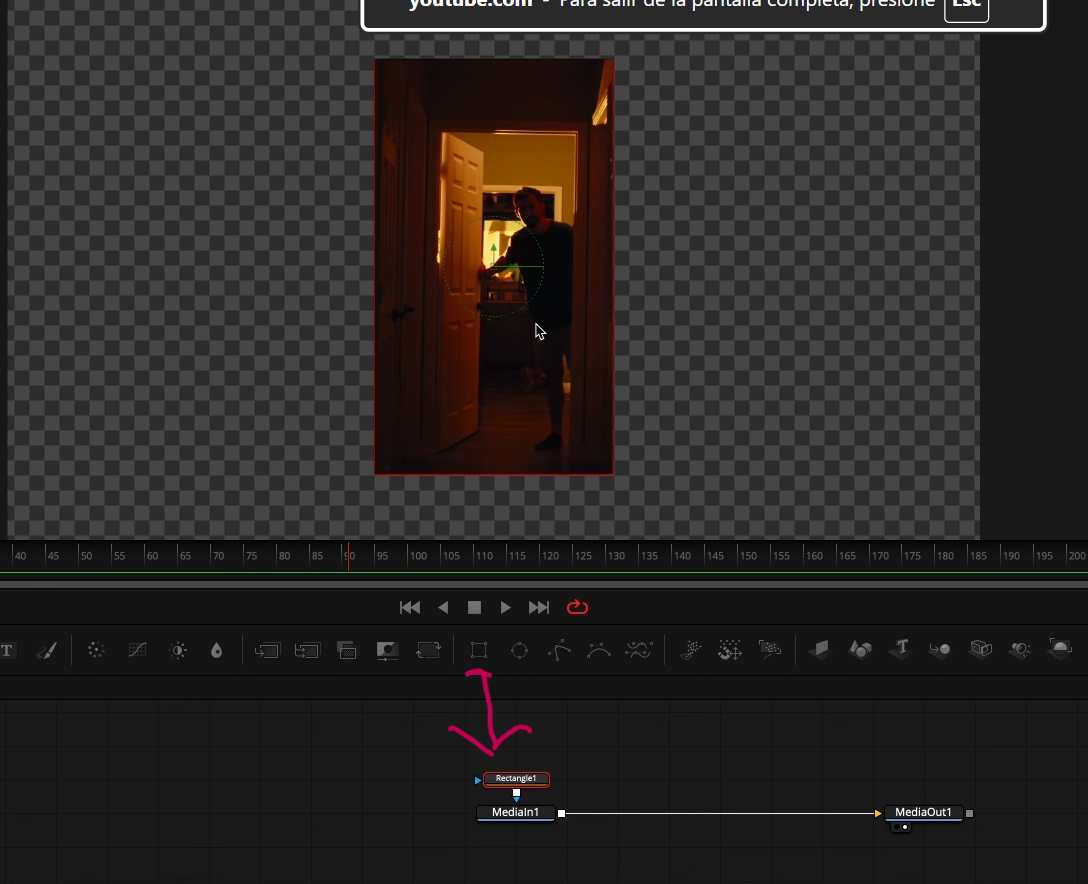
\includegraphics[width=1.0\textwidth]{assets/rectangle_puertas.png}
        \caption[Crear rectángulo]{Rectángulo sobre el clip de la puerta\\ \footnotesize Fuente: Elaboración propia}
        \label{fig:rectangle_puertas}
    \end{figure}

    \item \textbf{Aprovechamiento de espacio}
    
    Uno de los aspectos clave al incorporar múltiples clips sobre un clip base o envolvente es la correcta organización del espacio de trabajo. 
    Para ello, se utiliza una malla (\textit{grid}), que permite dividir la escena en celdas equivalentes, facilitando tanto la 
    distribución de los clips como su alineación.

    La adaptación de esta estructura se consigue mediante la incorporación de dos nodos adicionales sobre el nodo de entrada de 
    vídeo (\textit{MediaIn1}). Para ello, se selecciona dicho nodo y se utiliza el atajo de teclado \textit{Ctrl + Enter}, que 
    permite abrir el buscador de efectos. A continuación, se añaden, de forma secuencial, los nodos \textit{Transform} y \textit{Grid}.

    Una vez añadido el nodo \textit{Grid}, se procede a su configuración desde el panel situado en la parte derecha de la interfaz. 
    En este punto, se define el número de filas y columnas de la malla, estableciendo valores de 21 para \textit{Row Cells} y 
    25 para \textit{Column Cells}. Asimismo, el espaciado entre líneas (\textit{Major Line Spacing}) se ajusta a 0 con el objetivo de 
    evitar saturación visual y mejorar la precisión durante la edición.

    Dado que las líneas de la malla pueden resultar excesivamente gruesas, es conveniente reducir su intensidad para facilitar 
    la visualización del contenido asociado. Para ello, se accede al apartado \textit{Settings}, situado en la parte superior de 
    esta misma vista de configuración, y se ajusta el valor del atributo \textit{Blend} a 0.3.

    Finalmente, el nodo \textit{Transform} permite posicionar el clip dentro del lienzo de trabajo. Para ello, se selecciona 
    el nodo y se accede a su configuración en el panel derecho de la interfaz, donde se modifican los parámetros \textit{Center} y 
    \textit{Pivot}. De este modo, el clip puede alinearse correctamente con la malla definida (véase Figura~\ref{fig:ajuste_malla}).

    \begin{figure}[H]
        \centering
        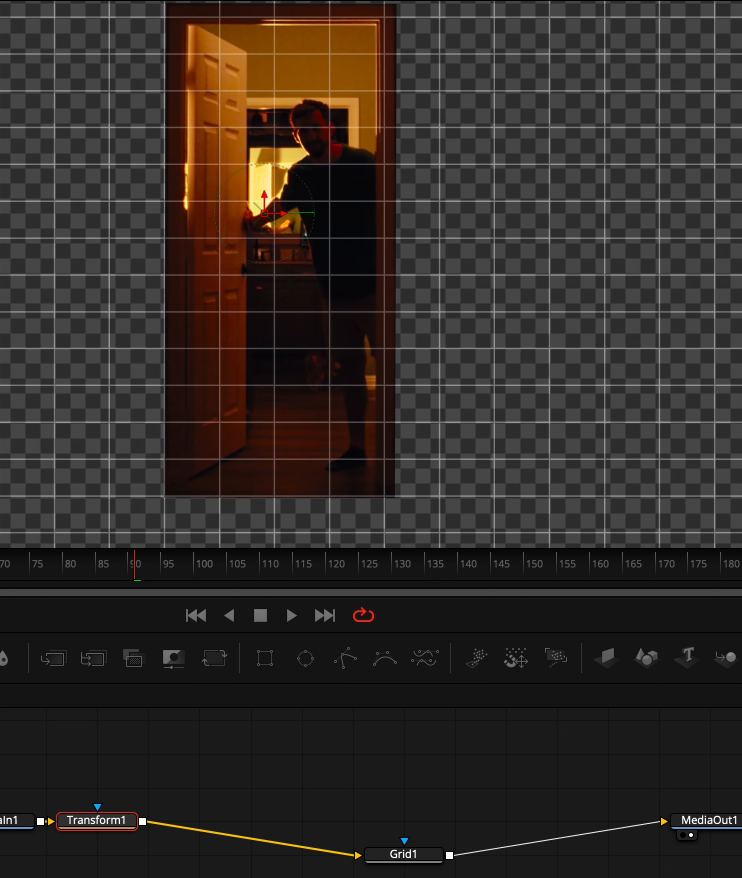
\includegraphics[width=0.8\textwidth]{assets/ajuste_malla.png}
        \caption[Ajuste malla]{Ajuste del clip en la malla\\ \footnotesize Fuente: Elaboración propia}
        \label{fig:ajuste_malla}
    \end{figure}
    
    \item \textbf{Repetición de contenido}
    
    Una vez configurada la base de trabajo, el siguiente paso consiste en replicarla tantas veces como permita el espacio disponible en 
    el lienzo, con el objetivo de generar el efecto de repetición deseado.

    Para ello, se emplea el nodo \textit{MultiMerge}, cuya funcionalidad permite combinar múltiples entradas multimedia en un único 
    resultado final. Este nodo será el encargado de agrupar todos los clips generados a partir de la estructura base.

    La incorporación del nodo \textit{MultiMerge} se realiza seleccionando el nodo \textit{Transform} previamente añadido y utilizando 
    el atajo \textit{Ctrl + Enter} para abrir el buscador de efectos. A continuación, se localiza y se añade dicho nodo.

    Posteriormente, con el fin de mantener la misma configuración en todos los clips duplicados, se agrupan los nodos \textit{Rectangle1}, 
    \textit{MediaIn1} y \textit{Transform1}. Para ello, se seleccionan de forma conjunta, se hace clic derecho y se elige la 
    opción \textit{Group}. Esta agrupación permite duplicar fácilmente la estructura mediante \textit{Ctrl + C} y \textit{Ctrl + V}, 
    favoreciendo además una organización más limpia del entorno de trabajo.

    Cada uno de los grupos generados debe conectarse al nodo \textit{MultiMerge}, que se encargará de procesarlos de forma conjunta. 
    A medida que se duplican los grupos, los clips comienzan a distribuirse sobre el lienzo, por lo que resulta fundamental mantener 
    un criterio de organización. Como recomendación, se sugiere dejar un margen de al menos una celda de la malla entre cada clip, con 
    el fin de preservar la claridad visual y evitar solapamientos (véase Figura~\ref{fig:loop_puertas}).

    \begin{figure}[H]
        \centering
        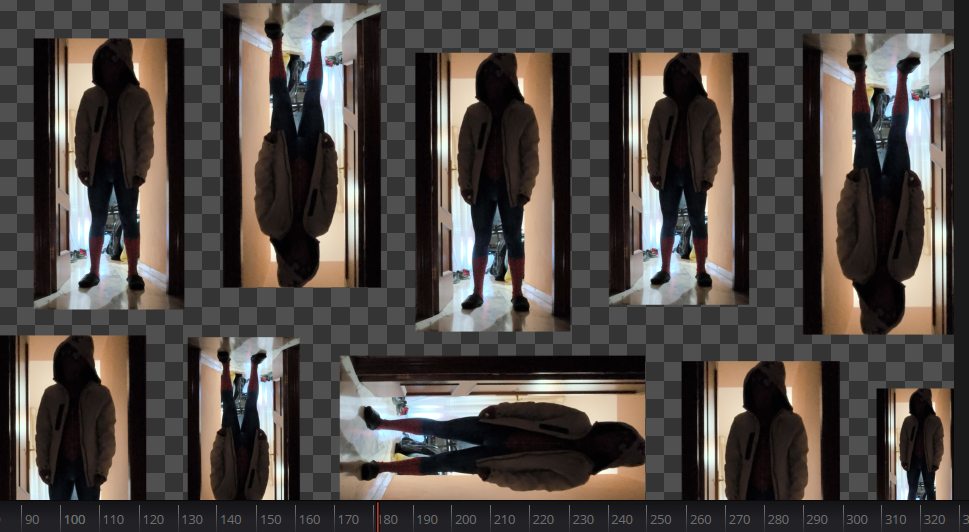
\includegraphics[width=0.8\textwidth]{assets/loop_puertas.png}
        \caption[Loop puertas]{Loop de puertas\\ \footnotesize Fuente: Elaboración propia}
        \label{fig:loop_puertas}
    \end{figure}
\end{enumerate}

\subsubsection{Dolly Zoom y Efecto estabilizador}
    
La incorporación del efecto \textit{Dolly Zoom} y Estabilizador tienen el objetivo de proporcionar ajustes de zoom combinando el movimiento 
físico de la cámara (dolly). Permite mantener el tamaño original del actor, mientras el fondo se comprime o se estira drásticamente, generando 
distorsión visual que genera sensación de alucinación, mareo, sorpera, entre otros.


\textbf{Pasos seguidos para la aplicación de este efecto:}
\begin{enumerate}[label=\arabic*.]
    \item \textbf{Configuración \textit{Dolly Zoom}}
    
    Tras haber importado e incorporado a la línea de tiempo el archivo multimedia sobre el que se va a trabajar, es necesario identificar 
    los instantes de tiempo inicial y final en los que se desea aplicar el efecto de aumento o disminución de zoom.

    Una vez identificados estos instantes clave, desde el apartado \textbf{Cut} (véase Sección~\ref{sec:modulos-trabajo}, 
    Figura~\ref{fig:modulos_trabajo}), se crean \textit{KeyFrames} en el instante inicial sobre los atributos \textit{Zoom} y 
    \textit{Position} desde el panel situado en la parte derecha de la interfaz. Este mismo procedimiento se repite para el instante final.

    A continuación, se procede a la búsqueda del efecto \textit{Shape Circle} desde el panel de \textbf{Efectos} (véase Figura~\ref{fig:seccion_efectos}). Una vez localizado, 
    se arrastra sobre el clip para incorporarlo, generando un círculo 2D superpuesto. Este efecto permite establecer un punto estático 
    de enfoque sobre una zona concreta del vídeo, independientemente de los movimientos de cámara o de velocidad.

    Para facilitar la configuración del efecto, se recomienda ajustar el valor de la propiedad \textit{Blend} a aproximadamente 0.2, 
    lo que añade transparencia al círculo y permite visualizar el contenido situado detrás.

    Finalmente, dado que el enfoque suele centrarse en un objeto concreto, es necesario ajustar tanto el tamaño como la posición del 
    círculo desde el panel de configuración, alineándolo con el elemento objetivo dentro del plano (véase Figura~\ref{fig:circulo_dolly}).

    \begin{figure}[H]
        \centering
        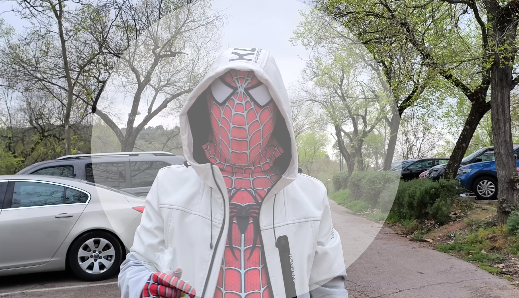
\includegraphics[width=0.6\textwidth]{assets/circulo_dolly.png}
        \caption[Circulo efecto dolly]{Círculo para efecto \textit{dolly}\\ \footnotesize Fuente: Elaboración propia}
        \label{fig:circulo_dolly}
    \end{figure}

    \begin{figure}[H]
        \centering
        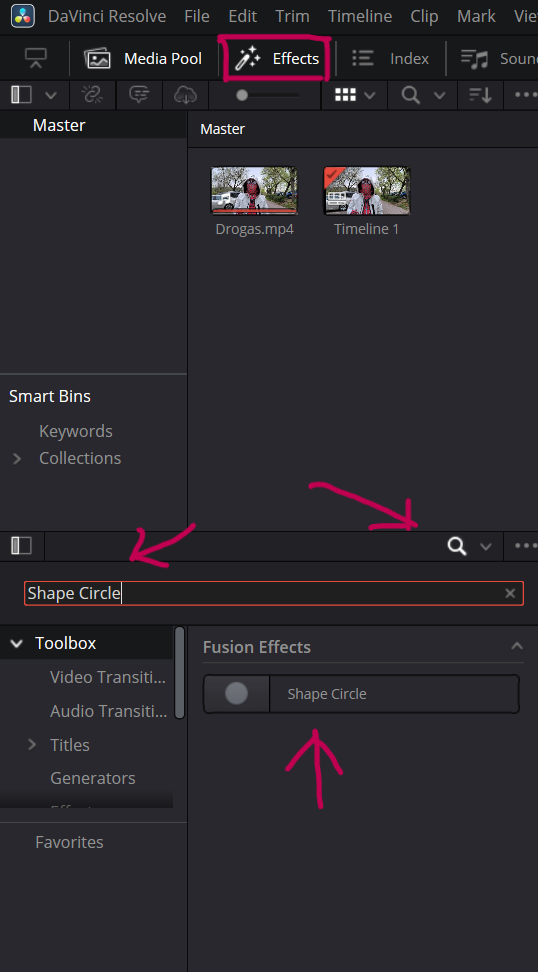
\includegraphics[width=0.5\textwidth]{assets/seccion_efectos.png}
        \caption[Seccion efectos]{Sección de efectos\\ \footnotesize Fuente: Elaboración propia}
        \label{fig:seccion_efectos}
    \end{figure}

    Finalmente, se deselecciona el efecto asociado al círculo en la sección \textit{Effects}, 
    con el fin de que no aparezca en el resultado final (véase Figura~\ref{fig:desactivar_circulo}).

    \begin{figure}[H]
        \centering
        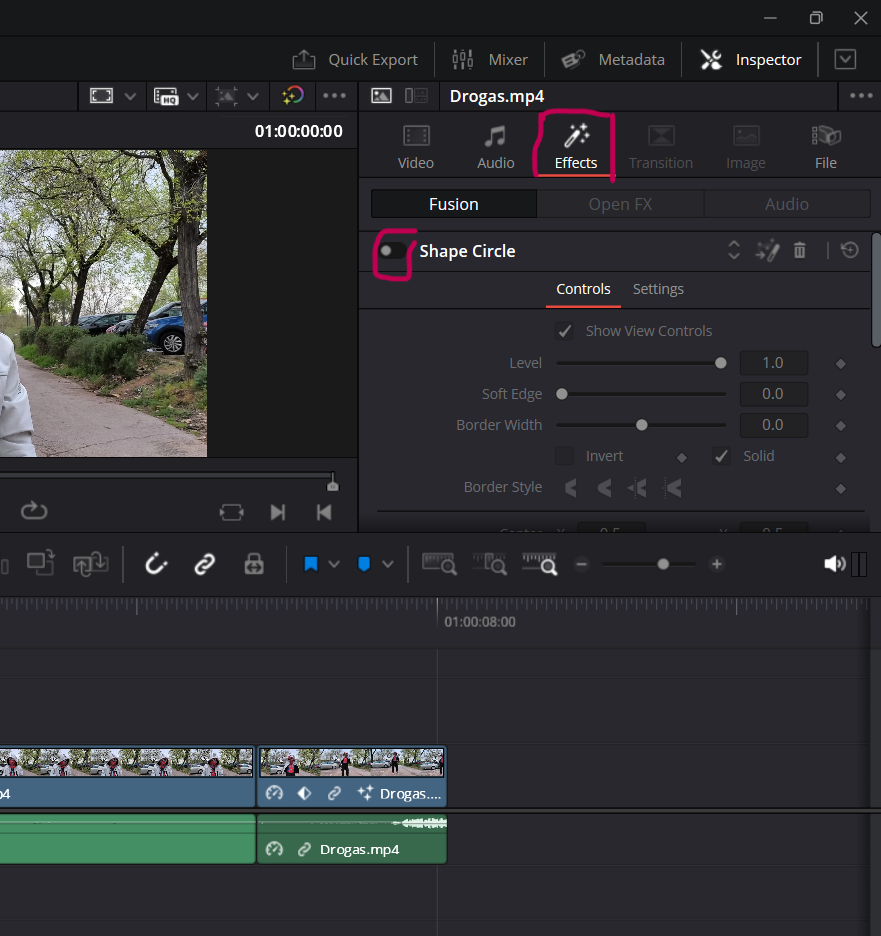
\includegraphics[width=0.5\textwidth]{assets/desactivar_circulo.png}
        \caption[Desactivar efecto]{Desactivar visualización efecto\\ \footnotesize Fuente: Elaboración propia}
        \label{fig:desactivar_circulo}
    \end{figure}

    \item \textbf{Configuración efecto estabilizador}
    
    La configuración de este efecto se realiza sobre la segunda fase del efecto \textit{dolly}, 
    también conocida como fase de desenfoque.

    Como se ha mencionado anteriormente, es necesario identificar los instantes de tiempo inicial 
    y final sobre el archivo multimedia en los que se desea aplicar el filtro. Asimismo, es importante 
    seleccionar intervalos en los que la cara de la persona o el objeto de interés no experimenten 
    cambios bruscos de posición, procurando que su movimiento sea lo más estable posible.

    Una vez definidas estas condiciones iniciales, se accede al apartado \textit{Color} 
    (véase Sección~\ref{sec:modulos-trabajo}, Figura~\ref{fig:modulos_trabajo}). En este entorno, 
    se utilizan las herramientas situadas justo debajo de la ventana de visualización del clip, 
    seleccionando la opción \textit{Tracker} (véase Figura~\ref{fig:estabilizador}). El objetivo de esta herramienta es permitir 
    la definición de una región de interés mediante un polígono de puntos que abarque aproximadamente 
    la cabeza de la persona o el objeto a seguir, facilitando así su detección y seguimiento por 
    parte del algoritmo.

    Tras seleccionar dicha herramienta, aparece una barra adicional con opciones más específicas. 
    En ella, se selecciona la opción \textit{Stabilizer}. A continuación, mediante el menú de los 
    tres puntos (...), se elige \textit{Classic Stabilizer}, lo que permite aplicar la estabilización 
    únicamente sobre la región previamente definida (véase Figura~\ref{fig:estabilizador}).

    Además, en la barra de herramientas asociada, se puede configurar el tipo de rastreo: 
    \textbf{por puntos} o \textbf{por nube de puntos}. Se recomienda utilizar el modo de nube 
    de puntos, ya que permite al algoritmo compensar posibles errores seleccionando puntos vecinos, 
    mejorando así la robustez del seguimiento. Asimismo, es conveniente activar la opción 
    \textit{Interactive Mode} (véase Figura~\ref{fig:estabilizador}, línea roja inferior), que genera una nube de puntos visible sobre el clip, facilitando 
    la comprensión y ajuste del comportamiento del algoritmo.

    Para definir la zona a rastrear, se utiliza la opción \textit{Insert}, situada a la 
    derecha de \textit{Interactive Mode}. Desde la vista del clip, se debe hacer clic y arrastrar 
    con el ratón para generar un rectángulo que \textcolor{importante}{debe} contener la región de 
    la cara o del objeto que se desea rastrear.

    Aunque se ha definido la zona de rastreo, el algoritmo puede perder precision debido a que siguen 
    existiendo puntos de rastreo fuera de la zona definida. Para eliminarlos, basta con selecciona la 
    opción situada a la derecha de \textit{Stabilizer}, llamada \textit{Clear All Tracking Points} y 
    volver a hacer clic en la opción \textit{Insert}.

    Finalmente, para comenzar con el registro de seguimiento, se debe seleccionar la opción 
    \textit{Track Forward and Reverse} (véase Figura~\ref{fig:estabilizador}, flecha roja superior), situada justo debajo del nombre de la ventana de herramientas 
    con la que se ha estado trabajando: \textit{Tracker - Window}.

    \begin{figure}[H]
        \centering
        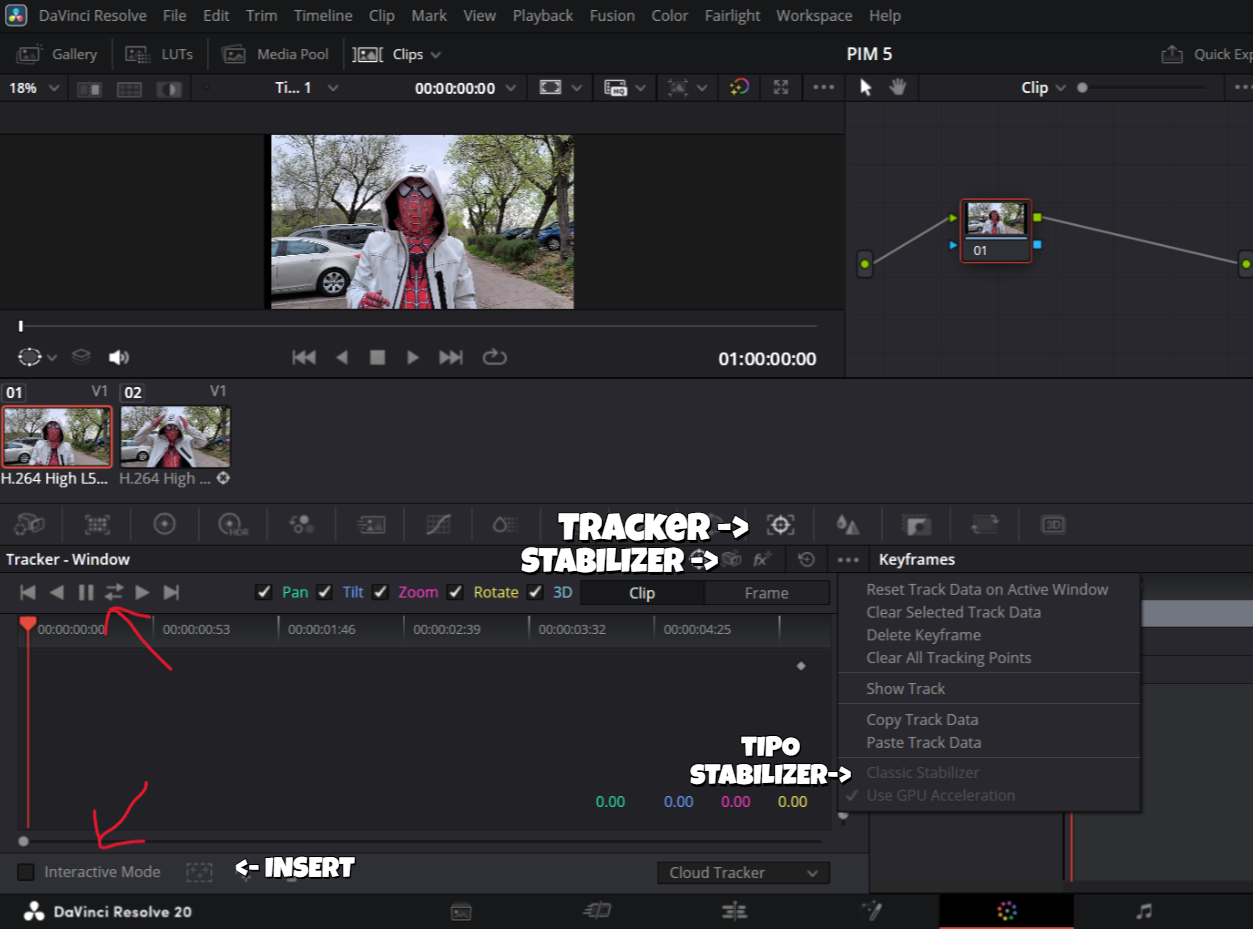
\includegraphics[width=1.0\textwidth]{assets/estabilizador.png}
        \caption[Config estabilización]{Opciones indicadas para configurar estabilizador\\ \footnotesize Fuente: Elaboración propia}
        \label{fig:estabilizador}
    \end{figure}
            

\end{enumerate}